\section{Introduction}
topological states and topological phenomena are rooted in quantum mechanics in an essential way: They are states of matter whose quantum mechanical wave functions are topologically nontrivial and distinct from trivial states of matter\par
a theme that emerged from spin-orbit-induced topological insulators is the interplay(interaction) between symmetry and topology. \par
Symmetries play an important role in the Landau-Ginzburg-Wilson framework of spontaneous symmetry breaking for the classification of different states of matter\par
topological insulators cannot be distinguished from ordinary, topologically trivial
insulators in terms of their symmetries and their topological
nontriviality cannot be detected by a local order parameter.\par
in making a distinction between spin-orbit-induced
topological insulators and ordinary insulators, time-reversal
symmetry is crucial.\par

\subsection{Overview of topological materials}
First, insulating electronic band structures can be categorized
in terms of topology\par
In the case of spin-orbit-induced topological insulators
the topological nontriviality is guaranteed by time-reversal
symmetry\par
Second, topological concepts can be applied to unconventional
superconductors and superfluids.\par
Third, nodal systems, such as semimetals and nodal superconductors,
can exhibit nontrivial band topology, even though the bulk gap closes at certain points in the Brillouin zone (BZ).\par

\section{Symmetries}

\subsection{general properties}
for a feminion system the animation and creation operator labels as $\hat{\Psi},\hat{\Psi}^{\dagger}$\par
\noindent 1.Time Reversal Symmetry $\hat{T}$
\[\hat{T}\Psi_I\hat{T}^{-1}=U_I^J\Psi_J\]
\[ \hat{T}i\hat{T}^{-1}=-i\]
$THT^{-1}=H$ implies that:
\[U_T^{\dagger}H^*U_T=+H\]
\noindent 2.Partical Hole Symmetry$\hat{C}$
\[C\Psi_IC^{-1}=(U_C^*)_I^J\Psi_J^{\dagger}\]
$CHC^{-1}=H$ implies that:
\[U_C^{\dagger}H^TU_C=-H\]
Hubbard Model on a bipartical lattice:
\[H=\sum_{ij}^{i\neq j}\sum_{\sigma}t_{ij}c_{i\sigma}^{\dagger}c_{j\sigma}-\mu\sum_i\sum_{\sigma}n_{i\sigma}+U\sum_i n_{i \uparrow}n_{i\downarrow}\] 
\noindent 3.Chiral Symmetry $\hat{S}$\par
\[\hat{S}=\hat{T}\hat{C}\]
\[S\Psi_IS^{-1}=(U_CU_T)_I^J\Psi_J^{\dagger}\]

\subsection{BdG system}
\noindent 1.Symmetry Class D:\par
using $\tau_1$ to stand for the pauli metric acting on Nambu Space:
\[\tau_1H^T\tau_1=-H\]
\noindent 2.Symmetry Class DIII:\par
\[\tau_1H^T\tau_1=-H\]
\[\sigma_2 H^*\sigma_2=H\]
\noindent 3.Symmetry Class A\par
The Hamitonian has unnconstraint $\Psi$ and $\Psi^\dagger$\par
\noindent 4.Symmetry Class AIII\par
the hamitonian satisfying a chiral symmetry.\par
\noindent 5.Symmetry class C\par
For the single-particle Hamiltonian H the π-rotation symmetries $U_{Si}^{\pi}$ lead to the condition:
\[\sigma_2H^T\sigma_2=-H\]
he ensemble of Hamiltonians satisfying this condition is
called symmetry class C.
\noindent 6.Symmetry class CI\par
\[\sigma_2H^T\sigma_2=-H\]
\[H^*=-H\]
\subsubsection{Symmetry classes of the tenfold way}
the nonunitary symmetries is concluded in figure \ref{fig:tenfold} which is called tenfold way of the symmetry class.
\begin{figure}
\begin{center}
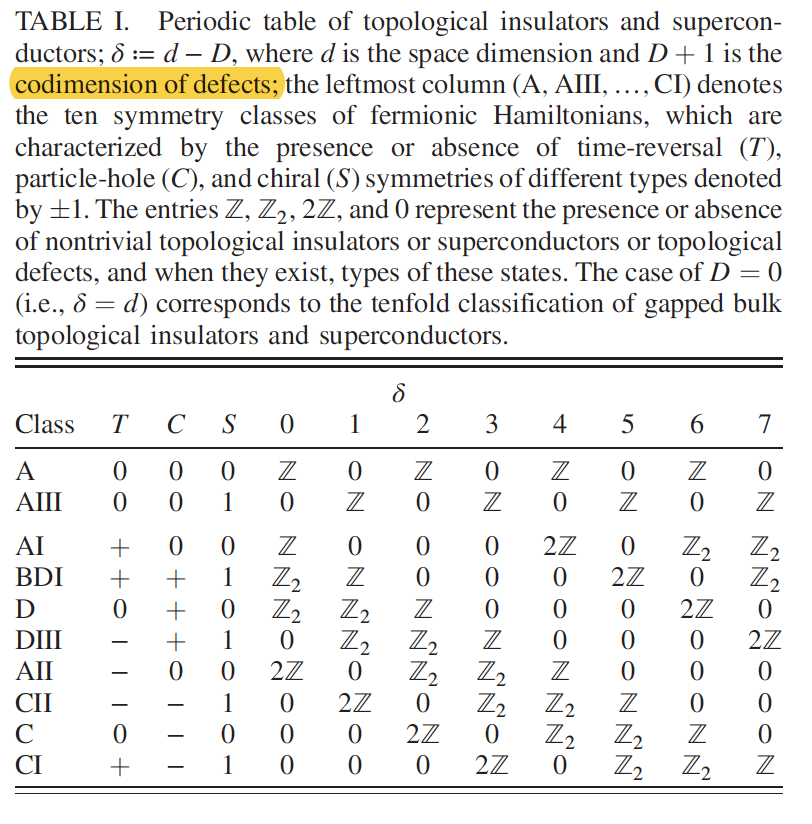
\includegraphics[height=10cm]{figures/tenfold.png}
\caption{Symmetry classes of the tenfold way}\label{fig:tenfold}
\end{center}
\end{figure}

\section{fully gapped free-fermion system and topological defects}
free fermion system is discribed by quadratic Bloch-BdG Hamiltonians:
\[\hat{H}=\sum_{r,r'}\hat{\Psi}_i^\dagger(r)H^{ij}(r,r')\hat{\Psi}_j(r')\]
and when asuming that $H(r,r')=H(r-r')$  we can make  fourier transformation and get $H(k)$.\par
we use the below hamitonian to discrib topological defects:
\[H_r(k)=H(k,r)\]
where the r is a parameter slowly modulate the Hamitonian and it includes spatial coordinates and/or a temporal parameter.Different defect Hamiltonians are distinguished by (i) the
AZ symmetry class s, (ii) the bulk dimension d, and (iii) the
defect codimension dc defined in terms of the dimension of
the defect $d_{defect}$ by
 \[d_c=d-d_{defect}\]
and we defined other parameters:
\[D=d_c-1\]
\[\delta=d-D\]
the ten symmetry classes can be divided to real AZ symmetry and complex AZ symmetry (where is no exisit of TRS PHS).for the eight real AZ symmetry ,it was shown that the classification of topological defects depends only on a single number
\[s-\delta=s-d+D ( mode 8)\]

\subsection{topological invariants}
the bloch wave function is defined in:
\[(k,r)\in BZ^d\times M^D\rightarrow S^{d+D}\]
\subsubsection{Primary series for s even: The Chern number}
For gapped topological phases and topological defects in
nonchiral classes (i.e., s is even), the Z-classified topologies
are characterized by the Chern number:
\[Ch_n=\frac{1}{n!}(\frac{i}{2\pi})^n\int_{BZ^d\times M^D}Tr(F^n)\]
where $n=\frac{d+D}{2}$ and F is the Berry Curvature:
\[F=dA+A^2\]
A is Berry Connection:
\[A^{\alpha \beta}(k,r)=\diracinner{u^{\alpha}}{du^{\beta}}\]
